\documentclass[a4paper,10pt]{scrreprt}
\usepackage[utf8]{inputenc}
\usepackage[german]{babel}
\usepackage{listings}
\usepackage{color}
\usepackage{graphicx}
\usepackage{hyperref}
\usepackage{xcolor}
\hypersetup{
    colorlinks,
    linkcolor={red!50!black},
    citecolor={blue!50!black},
    urlcolor={blue!80!black}
}
\definecolor{light-gray}{gray}{0.95}

\lstset{basicstyle=\ttfamily, breaklines=true, backgroundcolor=\color{light-gray}}
\title{EAS - Elektronisches AufrufSystem}
\subtitle{Handbuch}
\date{\today}
\author{Julian Hartig}

\begin{document}
\maketitle
\tableofcontents
\newpage
\chapter{Einleitung}
Das Elektronische AufrufSystem ist ein für Arztpraxen und vergleichbare Einrichtungen gedachtes Patientenaufrufsystem. Es bietet eine Aufrufansicht für das Wartezimmer sowie ein Kontrollinterface und auf Wunsch auch Interfaces für einzelne Räume, um die Raumbelegung nach außen zu signalisieren. 

Die Implementierung erfolgt in Python, somit ist das System auf allen von Python unterstützen Betriebssystemen lauffähig. Die jeweiligen Ansichten werden als Website geladen, sodass sie auf jedem Endgerät angezeigt werden könne, welches über einen Webbrowser und Netzwerkanbindung verfügt,
neben den Praxiscomputern beispielsweise also auch auf einem an einen Raspberry Pi angeschlossenen Monitor im Wartezimmer oder einem Tablet neben der Sprechzimmertür.

Das System kann grundsätzlich an jedes Praxisverwaltungssystem angebunden werden, welches die Ansteuerung von Drittsoftware über die GDT"=Schnittstelle unterstützt. Bei Praxisverwaltungssystem, die den Patientenaufruf über eine BDT"=Aufrufschnittstelle unterstützen (wie z.B. Medical Office der Fa. Indamed)
kann der aktuell in einem Raum befindliche Patient auch über das EAS-Kontrollinterface per Klick im Praxisverwaltungssystem aufgerufen werden. Das für die Kommunikation verwendete, offene WAMP-Protokoll erlaubt außerdem prinzipiell eine noch engere Integration des Praxisverwaltungssystem, wenn vom Hersteller 
gewünscht.

\chapter{Installation}
\section{Grundsätzliche Systemvoraussetzungen}
\section{Server}
Zum Betrieb des Servers ist die Installation des kostenlosen Open-Source Websocket-Routers \texttt{crossbar.io} erforderlich. Eine passende Konfiguration findet sich im Repository von EAS.
Außerdem werden neben einem lauffähigen Python-Interpreter (v2.7.x) noch die Python-Packages \texttt{autobahn} und \texttt{peewee} mit ihren Abhängigkeiten benötigt. Diese lassen sich, ebenso wie \texttt{crossbar.io} komfortabel über
das Python-Paketverwaltungssystem \texttt{pip} installieren.

Bezüglich einer Anleitung zum Starten von \texttt{crossbar.io} beim Systemstart sei an dieser Stelle auf die Dokumentation von \texttt{crossbar.io} verwiesen. Es muss außerdem das Python-Skript \texttt{server/easserver.py} aus dem Repository ausgeführt werden.
Die EAS-Datenbank wird unter dem Dateinamen \texttt{eas.db} im Arbeitsverzeichnis erwartet. Existiert diese Datei dort nicht, so wird sie beim Ausführen von \texttt{easserver.py} automatisch erzeugt und die notwendigen Tabellen angelegt.

Der Server ist standardmäßig so konfiguriert, dass er eingehende Anfragen auf Port \texttt{8080} erwartet. Soll ein abweichender Port verwendet werden, so muss eine entsprechende Änderung in der Datei \texttt{.crossbar/config.json} sowie im Kopfbereich von \texttt{easserver.py} erfolgen.

\subsection{Tonsignal bei Patientenaufruf}
\label{ssec:tonsignal}
Die Wartezimmeransicht unterstützt die Ausgabe eines Tonsignals beim Aufruf eines Patienten. Hierfür muss eine Datei mit dem Namen \texttt{bell.mp3} im Verzeichnis \texttt{webroot} abgelegt werden, die den gewünschten Ton enthält. Das Internet hält hierzu zahlreiche kostenlos verwendbare Klänge bereit.

\section{Client}
\subsection{Webansichten}
Die Ausgabe der Wartezimmer-, Kontroll- und Raumbelegungsansicht setzt nur einen Webbrowser voraus. In diesem muss dann eine der folgenden Adressen aufgerufen werden:
\begin{lstlisting}
  http://<server-ip>:<server-port>/wartezimmer.html
  http://<server-ip>:<server-port>/control.html
\end{lstlisting}

\subsection{PVS-Anbindung}
Für die Anbindung des Praxisverwaltungssystems sind die Skripte im Verzeichnis \texttt{clients} vorgesehen. 
\subsubsection{eas-populate-room.py}
Mit diesem Skript kann das Praxisverwaltungssystem einen Patienten aufrufen. Es benötigt das Python-Paket \texttt{autobahn} (s.o.).

Das Praxisverwaltungssystem muss hierbei so konfiguriert werden, dass das Skript folgendermaßen aufgerufen wird:
\begin{lstlisting}
 $ eas-populate-room.py <server-ip>:<server-port> 
 C:\Pfad\zur\Datei.gdt "Name des Zimmers"
\end{lstlisting}
Als Testkennung ist \texttt{CALL} zu übergeben. Soll ein Sprechzimmer freigegeben werden, ohne dass ein neuer Patient aufgerufen werden soll, so ist \texttt{LEAVE} zu übergeben. Die in der GDT-Datei übermittelten Patientendaten werden dann ignoriert.

Für das Programm Medical Office bietet sich hier die Konfiguration einzelner Aufträge für jedes vorhandene Sprechzimmer im Datenpflegesystem an. Diese Aufträge können dann mit Schaltern in der Schalterleiste verknüpft werden,
sodass der aktuell in Medical Office aufgerufene Patient über EAS in das entsprechende Zimmer bestellt wird.

\subsubsection{eas-create-gdt.py}
Dieses Skript dient als Hilfsskript, um einen automatischen Patientenaufruf im Praxisverwaltungssystem über eine BDT"=Datei zu ermöglichen, sofern dies vom Praxisverwaltungssystem unterstützt wird. Hierzu muss der verwendete Webbrowser so konfiguriert werden,
dass er beim Klicken eines \texttt{easpatient}-Links aus der Kontrollansicht das Skript wie folgt aufruft:
\begin{lstlisting}
 $ eas-create-gdt.py C:\Pfad\zur\Aufrufdatei.bdt Patientennummer
\end{lstlisting}
Die Patientennummer darf hierbei auch noch das vorangestellte \texttt{easpatient:} enthalten, dieses wird vom Skript dann automatisch vor der Übergabe der Patientennummer an das Praxisverwaltungssystem entfernt.

Konfigurationsanleitungen für benutzerspezifische Linkprotokolle finden sich auf den Webseiten der Browserhersteller. Für Microsoft Windows ist (auch) eine zentrale Konfiguration über die Registry möglich.

\chapter{Konfiguration}
Die Konfiguration von EAS erfolgt webbasiert über das Kontrollinterface:
\begin{lstlisting}
 http://<server-ip>:<server-port>/control.html
\end{lstlisting}

\begin{figure}[h]
 \centering
 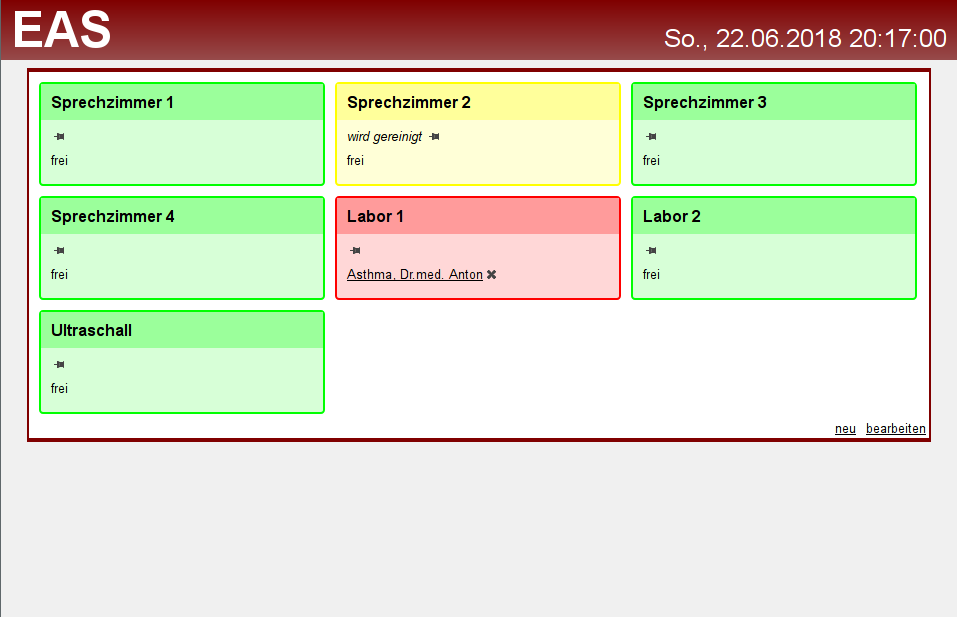
\includegraphics[width=\textwidth]{./Screenshot-Control.png}
 % Screenshot-Control.png: 0x0 pixel, 300dpi, 0.00x0.00 cm, bb=
 \label{controlinterface}
 \caption{Kontrollinterface}
\end{figure}

\section{Neuen Raum anlegen}
Mit Klick auf den Link \glqq{}neu\grqq{} können neue Räume angelegt werden. Es öffnet sich ein Fenster zur Eingabe des Raumnamens und der Raumpriorität. Die Raumpriorität dient hierbei zur Bestimmung der Anordnung der Räume in der Kontrollansicht.
Der Raum mit der niedrigsten Priorität erscheint oben links, der Raum mit der höchsten Priorität unten rechts.

\section{Raum bearbeiten}
Zum Bearbeiten von Räumen muss der Link \glqq{}bearbeiten\grqq{} angeklickt werden. Anschließend werden über jedem Raum ein Eingabefeld für die Priorität sowie ein Button zum Löschen des Raumes eingeblendet. Die eingegebene Priorität wird bei Verlassen des Eingabefeldes oder Druck von \texttt{<ENTER>}
automatisch gespeichert.

Der Bearbeitungsmodus kann mit einem erneuten Klick auf den \glqq{}bearbeiten\grqq{}-Link verlassen werden.

\section{Nachricht hinterlegen}
Über einen Klick auf die Pinnadel unterhalb des Raumnamens kann eine raumbezogene Nachricht hinterlegt werden. Diese wird dann neben der Pinnadel angezeigt, der Raum verfärbt sich gelb (siehe Raum \glqq{}Sprechzimmer 2\grqq{} Screenshot S. \pageref{controlinterface}).

\section{Raum leeren}
Ist ein Raum durch einen Patienten belegt, so kann der Raum durch Klick auf das neben dem Patientennamen dargestellte Kreuz freigegeben werden. Ein belegter Raum wird in der Kontrollansicht rot dargestellt (siehe Raum \glqq{}Labor 1\grqq{} Screenshot S. \pageref{controlinterface}).

Ein leerer Raum erscheint in der Kontrollansicht grün.

\chapter{Wartezimmeransicht}
Die Wartezimmeransicht wird über diese Adresse aufgerufen:
\begin{lstlisting}
 http://<server-ip>:<server-port>/wartezimmer.html
\end{lstlisting}

In der Wartezimmeransicht werden bis zu acht Patienten untereinander angezeigt mit den jeweiligen Räumen, in die die Patienten sich begeben sollen. Der aktuellste Aufruf erscheint jeweils ganz unten in der Liste und blinkt für ca. 20 Sekunden auf. Auf Wunsch kann auch ein Signalton abgespielt werden,
wenn ein neuer Aufruf erscheint (siehe Abschnitt \ref{ssec:tonsignal}).

\begin{figure}[h]
 \centering
 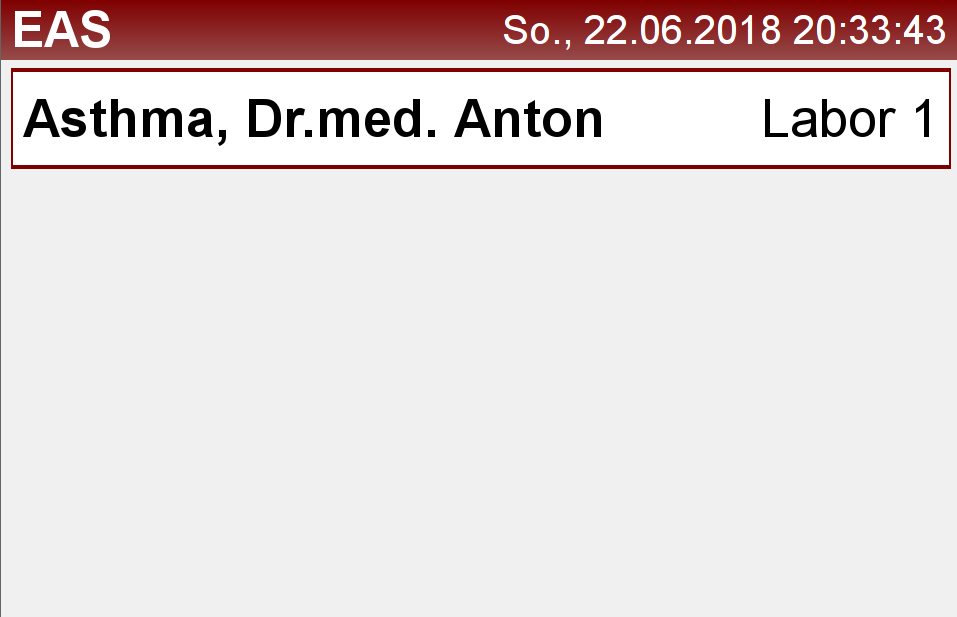
\includegraphics[width=\textwidth]{./Screenshot-Wartezimmer.png}
 % Screenshot-Control.png: 0x0 pixel, 300dpi, 0.00x0.00 cm, bb=
 \label{controlinterface}
 \caption{Wartezimmeransicht}
\end{figure}

Sind die acht Einträge erreicht, so wird bei neuen Einträgen der jeweils älteste Eintrag von der Liste entfernt. Außerdem werden Patienten aus der Liste entfernt, die den entsprechenden Raum verlassen haben. Dies sorgt dafür, dass die Liste so übersichtlich wie möglich bleibt.

\chapter{Anpassung des Designs}
Durch entsprechende Bearbeitung der unter \texttt{webroot} befindlichen CSS-Dateien kann das Aussehen der EAS-Ansichten schnell und einfach an das Corporate Design der Praxis angepasst werden.

\appendix
\chapter{Lizenzinformationen}
Die EAS-Software steht unter der GPLv3. Der vollständige Lizenztext kann unter \texttt{https://www.gnu.org/licenses/gpl-3.0.de.html} eingesehen werden.

\end{document}
